\documentclass[a4paper,11pt]{article}

\usepackage[T1]{fontenc}
\usepackage[utf8]{inputenc}
\usepackage{graphicx}
\usepackage{xcolor}
\usepackage{amsmath,amssymb,amsthm}
\usepackage{enumerate}
\usepackage{hyperref}
\usepackage{multicol}
\usepackage{tikz}
\usepackage[force,almostfull]{textcomp}
\usepackage{geometry}
\usepackage{longtable}

\setcounter{secnumdepth}{4}

\graphicspath{ {./images/} }

\definecolor{linkcolour}{rgb}{0,0.2,0.6}
\hypersetup{colorlinks,breaklinks,urlcolor=linkcolour, linkcolor=linkcolour}

\geometry{total={210mm,297mm},
left=25mm,right=25mm,%
bindingoffset=0mm, top=20mm,bottom=20mm}

\renewcommand*\sfdefault{phv}
\renewcommand\familydefault{\sfdefault}

\newcommand*{\TitleFont}{%
      \usefont{\encodingdefault}{\sfdefault}{b}{n}%
      \fontsize{20}{22}%
      \selectfont}


\linespread{1.3}

\newcommand{\linia}{\rule{\linewidth}{0.5pt}}

% custom theorems if needed
\newtheoremstyle{mytheor}
    {1ex}{1ex}{\normalfont}{0pt}{\scshape}{.}{1ex}
    {{\thmname{#1 }}{\thmnumber{#2}}{\thmnote{ (#3)}}}

\theoremstyle{mytheor}
\newtheorem{defi}{Definition}

% my own titles
\makeatletter
\renewcommand{\maketitle}{
\begin{center}
\vspace{2ex}
{\huge \textsc{\@title}}
\vspace{1ex}
\\
\linia\\
\@author \hfill \@date
\vspace{4ex}
\end{center}
}
\makeatother
%%%

% custom footers and headers
\usepackage{fancyhdr}
\pagestyle{fancy}
\lhead{}
\chead{}
\rhead{}
\lfoot{Assignment: Booting(1) }
\cfoot{}
\rfoot{Page \thepage}
\renewcommand{\headrulewidth}{0pt}
\renewcommand{\footrulewidth}{0pt}
%

% code listing settings
\usepackage{listings}
\lstset{
    basicstyle=\ttfamily\small,
    aboveskip={1.0\baselineskip},
    belowskip={1.0\baselineskip},
    columns=fixed,
    extendedchars=true,
    breaklines=true,
    tabsize=4,
    prebreak=\raisebox{0ex}[0ex][0ex]{\ensuremath{\hookleftarrow}},
    frame=lines,
    showtabs=false,
    showspaces=false,
    showstringspaces=false,
    keywordstyle=\color[rgb]{0.627,0.126,0.941},
    commentstyle=\color[rgb]{0.133,0.545,0.133},
    stringstyle=\color[rgb]{01,0,0},
    numbers=left,
    numberstyle=\small,
    stepnumber=1,
    numbersep=10pt,
    captionpos=t,
    escapeinside={\%*}{*)}
}

%%%----------%%%----------%%%----------%%%----------%%%

\begin{document}

\title{\TitleFont Assignment: Booting(1) }

\author{Emil Sharifulllin, Innopolis University}

\date{\today}

\maketitle

\section{Installation}

\subsection{Troubleshooting}
The couple of troubles was occured during the installation process.

\subsubsection{Legacy PXE booting}
At the first trying installation process was interrupted by error. Following information was printed on the screen.

\begin{lstlisting}
PXE-E79: NBP is too big to fit in free base memory
PXE-M0F: Exiting Intel Boot Agent.
\end{lstlisting}
After googling I found a \href{https://social.technet.microsoft.com/Forums/windows/en-US/dc31331e-605d-420a-b827-9bfb745de633/pxee79-nbp-is-too-big-to-fit-in-free-base-memory?forum=winserversetup}{forum} with discussion about this problem, but most of methods, described in it not worked for me. The last message on it was useful for me. In this message was said that solution can be in choosing non-legacy way of booting. In BIOS I found option to boot in UEFI mode and it solved problem.

\subsection{Questions after Install}
\subsubsection{}

\textbf{(a) What is UEFI PXE booting?}\\
The Unified Extensible Firmware Interface (UEFI) is a specification that defines a software interface between an operating system and platform firmware.\\UEFI PXE(Preboot Execution Environment) is a computer booting environment that allows to boot operating system via network interface.\\
\textbf{(b) How does it work?}\\
PXE booting contain following steps:
\begin{enumerate}
    \item Network interface loads pxelinux loader.
    \item pxelinux sends request to DHCP server and receives own ip address and ip address of TFTP server.
    \item pxelinux requests Linux kernel and initrd image from TFTP server.
    \item When kernek is downloaded it starts to work.
    \item Linux kernel requests from DHCP server own ip address, NFS server address and root filesystem location on hard disk.
    \item Linux kernel mounts root filesystem.
    \item Linux kernel calls /sbin/init

\end{enumerate}
\textbf{(c) How does it compare to booting from the hard disk?}\\
PXE allows you to boot via network and you and it's not needed in booting disks or flash drive to install OS. If you boot from disk, UEFI try to find OS loader in /efi/boot/ folder on disk.

\subsubsection{}
\textbf{(a) What is GPT?}\\
GPT(GUID Partition Table) is a standard for the layout of the partition table on a physical storage device, such as a hard disk drive or solid-state drive, using globally unique identifiers (GUID).\\
\textbf{(b) What is its layout?}\\
GPT headers is stored at 1 - 34 and at -1 - (-34) LBA sectors.\\

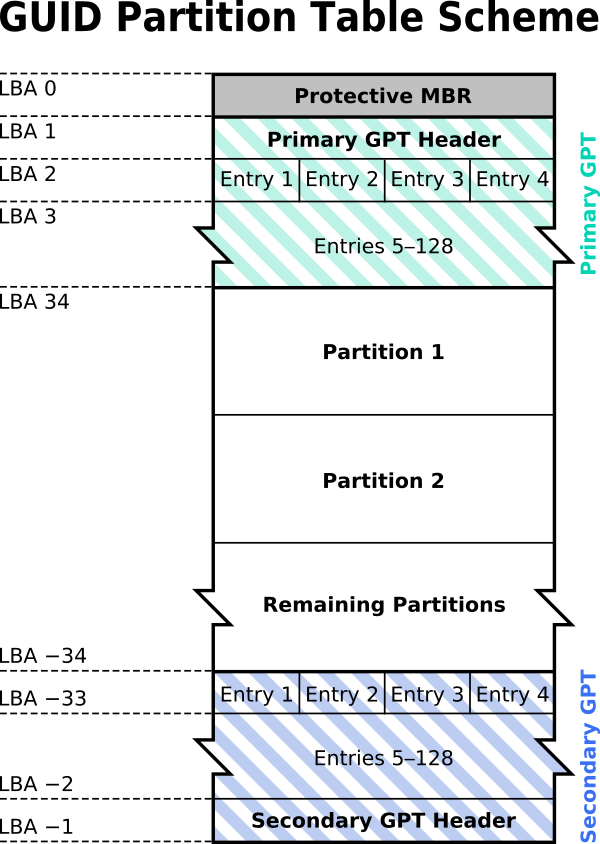
\includegraphics{gpt.png}\\
\textbf{(c) What can you do with it?}\\
It needed to store information about partitions and to tell UEFI what to boot.

\subsubsection{}
\textbf{(a) What is gdisk?}\\
gdisk is an utillity that allows you to manipulate with disk partition tables.
\textbf{(b) How does it work?}\\
When gdisk starts to work it scans disk and tries to find partition tables. gdisk can understand four type of partitions tables: MBR, BSD, APM, GPT. After defining storage gdisk parse partitions table and print information from in to console.\\
\textbf{(c) What can you do with it}\\
gdisk can help you to get information about your partition tables and partitions and can backup and restore partition tables. Here you can find all functions of gdisk: \\
\begin{itemize}
  \item back up GPT data to a file
  \item change a partition's name
  \item delete a partition
  \item show detailed information on a partition
  \item list known partition types
  \item add a new partition
  \item create a new empty GUID partition table (GPT)
  \item print the partition table
  \item recover and transform GPT
  \item change a partition's type code
  \item verify disk
  \item write table to disk
\end{itemize}

\subsubsection{}
\textbf{(a) What is Protective MBR and why is it in the GPT?}\\
Old systems, which uses BIOS instead of UEFI cannot understand GPT and because that can break disk partitioning. For this purposes GPT designers invented special protective mechanism that called Protective MBR. BIOS expect to find MBR at first LBA so when GPT is created it creates MBR with empty code sections and only one inactive partition that represents whole GPT disk.

\section{Partitions}

\subsection{MBR \& GPT}

\subsubsection{MBR}

Protective Master Boot Record is defined in first 512 bytes. It is needed to provide compability bith BIOS based systems such like a IBM PC. It define information about exactly one partition with System ID 0xEE and contain following data:

\begin{lstlisting}
00000000:  0000 0000 0000 0000 0000 0000 0000 0000 0000 0000 0000 0000 0000 0000 0000 0000
00000020:  0000 0000 0000 0000 0000 0000 0000 0000 0000 0000 0000 0000 0000 0000 0000 0000
00000040:  0000 0000 0000 0000 0000 0000 0000 0000 0000 0000 0000 0000 0000 0000 0000 0000
00000060:  0000 0000 0000 0000 0000 0000 0000 0000 0000 0000 0000 0000 0000 0000 0000 0000
00000080:  0000 0000 0000 0000 0000 0000 0000 0000 0000 0000 0000 0000 0000 0000 0000 0000
000000a0:  0000 0000 0000 0000 0000 0000 0000 0000 0000 0000 0000 0000 0000 0000 0000 0000
000000c0:  0000 0000 0000 0000 0000 0000 0000 0000 0000 0000 0000 0000 0000 0000 0000 0000
000000e0:  0000 0000 0000 0000 0000 0000 0000 0000 0000 0000 0000 0000 0000 0000 0000 0000
00000100:  0000 0000 0000 0000 0000 0000 0000 0000 0000 0000 0000 0000 0000 0000 0000 0000
00000120:  0000 0000 0000 0000 0000 0000 0000 0000 0000 0000 0000 0000 0000 0000 0000 0000
00000140:  0000 0000 0000 0000 0000 0000 0000 0000 0000 0000 0000 0000 0000 0000 0000 0000
00000160:  0000 0000 0000 0000 0000 0000 0000 0000 0000 0000 0000 0000 0000 0000 0000 0000
00000180:  0000 0000 0000 0000 0000 0000 0000 0000 0000 0000 0000 0000 0000 0000 0000 0000
000001a0:  0000 0000 0000 0000 0000 0000 0000 0000 0000 0000 0000 0000 0000 0000 0000 0000
000001c0:  0100 eefe ffff 0100 0000 af6d 7074 0000 0000 0000 0000 0000 0000 0000 0000 0000
000001e0:  0000 0000 0000 0000 0000 0000 0000 0000 0000 0000 0000 0000 0000 0000 0000 55aa


\end{lstlisting}

This binary data can be divided into following pieces:

\begin{tabular}{| p{3cm} | p{12cm} |} \hline
  0000h - 01BDh & \textbf{Loader code} - is set to null because loader is not needed for disk with GTP\\ \hline
  01BEh - 01CDh & \textbf{First partition} - containt information about first partition on disk wiil be covered later.\\ \hline
  01DEh - 01FDh & \textbf{Information about three another partitions} - is set to null because protective MBR can define only one partition.\\ \hline
  01FEh - 01FFh & \textbf{Signature} - Must be 55h AAh to satisfy correctness of MBR.\\ \hline
\end{tabular}

\paragraph{GPT partition}

Firs partition in Protective MBR must contain data about pseudo GPT partition
\begin{lstlisting}
000001b0:  0000 0000 0000 0000 0000 0000 0000 0000 0100 eefe ffff 0100
000001c8:  0000 af6d 7074 0000 0000 0000 0000 0000 0000 0000 0000 0000
\end{lstlisting}

This bloc of binary data can be interpreted as follows: 

\begin{tabular}{| p{3cm} | p{2cm} | p{10cm} |} \hline
  Data location in bloc & Value & Description\\ \hline
  0000 - 0001 & 00h & \textbf{Drive status} - Drive is inactive\\ \hline
  0001 - 0004 & 00h 01h 00h 00h & \textbf{Partition start address} - First sector of partition is at header 0, sector 1, cylinder 0\\ \hline
  0004 - 0005 & EEh & \textbf{Partition type code} - It means that partition is GPT\\ \hline
  0005 - 0008 & FEh FFh FFh & \textbf{Partition end address} - It means that last sector of bartition is at LBA FEh FFh FFh \\ \hline
  0008 - 0012 & 01h 00h 00h 00h & \textbf{First Absolute sector} - LBA of first absolute sector in the partition is 1 \\ \hline
  0012 - 0016 & AFh 6Dh 70h 74h & \textbf{Number of sectors} - this partition contains 1953525167 sectors\\ \hline
\end{tabular}

\subsubsection{GPT}
    GPT starts at 512'th byte or LBA 1 of hard drive and contain following header data: 

\begin{lstlisting}
00000200:  4546 4920 5041 5254 0000 0100 5c00 0000 91d3 def2 0000 0000 0100 0000 0000 0000
00000220:  af6d 7074 0000 0000 2200 0000 0000 0000 8e6d 7074 0000 0000 bcda e6e8 d5cf 3e46
00000240:  8427 8cb5 dc68 c1d9 0200 0000 0000 0000 8000 0000 8000 0000 4e44 3a1a 0000 0000
00000260:  0000 0000 0000 0000 0000 0000 0000 0000 0000 0000 0000 0000 0000 0000 0000 0000
00000280:  0000 0000 0000 0000 0000 0000 0000 0000 0000 0000 0000 0000 0000 0000 0000 0000
000002a0:  0000 0000 0000 0000 0000 0000 0000 0000 0000 0000 0000 0000 0000 0000 0000 0000
000002c0:  0000 0000 0000 0000 0000 0000 0000 0000 0000 0000 0000 0000 0000 0000 0000 0000
000002e0:  0000 0000 0000 0000 0000 0000 0000 0000 0000 0000 0000 0000 0000 0000 0000 0000
00000300:  0000 0000 0000 0000 0000 0000 0000 0000 0000 0000 0000 0000 0000 0000 0000 0000
00000320:  0000 0000 0000 0000 0000 0000 0000 0000 0000 0000 0000 0000 0000 0000 0000 0000
00000340:  0000 0000 0000 0000 0000 0000 0000 0000 0000 0000 0000 0000 0000 0000 0000 0000
00000360:  0000 0000 0000 0000 0000 0000 0000 0000 0000 0000 0000 0000 0000 0000 0000 0000
00000380:  0000 0000 0000 0000 0000 0000 0000 0000 0000 0000 0000 0000 0000 0000 0000 0000
000003a0:  0000 0000 0000 0000 0000 0000 0000 0000 0000 0000 0000 0000 0000 0000 0000 0000
000003c0:  0000 0000 0000 0000 0000 0000 0000 0000 0000 0000 0000 0000 0000 0000 0000 0000
000003e0:  0000 0000 0000 0000 0000 0000 0000 0000 0000 0000 0000 0000 0000 0000 0000 0000
\end{lstlisting}

\begin{longtable}{| p{3cm} | p{2cm} | p{10cm} |} \hline
  Data location & Value & Description\\ \hline
  0000 - 0008 & 45h 46h 49h 20h 50h 41h 52h 54h & \textbf{Signature} - "EFI PART"\\ \hline
  0008 - 0012 & 00h 00h 01h 00h & \textbf{Revision} - GPT version is 1.0\\ \hline
  0012 - 0016 & 5Ch 00h 00h 00h & \textbf{Header size} - in Little endian == 92 bytes\\ \hline
  0016 - 0020 & 91h D3h DEh F2h & \textbf{Cyclic redundancy check-32} - error-detecting code of header\\ \hline
  0020 - 0024 & 00h 00h 00h 00h & \textbf{Reserved} - must contain zero\\ \hline
  0024 - 0032 & 01h 00h 00h 00h 00h 00h 00h 00h & \textbf{Current LBA} - location of this copy of header is 1 LBA (in little endian)\\ \hline
  0032 - 0040 & AFh 6Dh 70h 47h 00h 00h 00h 00h & \textbf{Backup LBA} - LBA of header of bacup GPT is 1953525167 LBA\\ \hline
  0040 - 0048 & 22h 00h 00h 00h 00h 00h 00h 00h & \textbf{First usable LBA} - First partition starts at 34'th LBA\\ \hline
  0048 - 0056 & 8Eh 6Dh 70h 47h 00h 00h 00h 00h & \textbf{Last usable LBA} - Last partition ends at 1953525134 LBA\\ \hline
  0056 - 0072 & BCh DAh E6h E8h D5h CFh 3Eh 46h 84h 27h 8Ch B5h DCh 68h C1h D9h & \textbf{Disk GUID} - unigue ID of disk is E8E6DABC-CFD5-463E-8427-8CB5DC68C1D9\\ \hline
  0072 - 0080 & 02h 00h 00h 00h 00h 00h 00h 00h & \textbf{Starting LBA of array of partition entrie} - Laways must be 2 for primary GPT\\ \hline
  0080 - 0084 & 80h 00h 00h 00h & \textbf{Number of partition entries in array} - \\ \hline
  0084 - 0088 & 80h 00h 00h 00h & \textbf{Size of a single partition entry} - usually 80h or 128\\ \hline
  0088 - 0092 & 4Eh 44h 3Ah 1Ah & \textbf{CRC32} - Partitions array error-detecting code\\ \hline
  0092 - 0512 & 00h 00h ... & \textbf{Reserved} - Must contain zeroes\\ \hline


\end{longtable}

\paragraph{GPT entries}
Hard disk contain three partitions and so fourth entry is filled with zeroes. 

\subparagraph{First entry} First entry data:
\begin{lstlisting}
00000400:  2873 2ac1 1ff8 d211 ba4b 00a0 c93e c93b 97a2 60a7 3cb8 9349 83d5 b2e3 8ed9 b45f
00000420:  0008 0000 0000 0000 ff07 1000 0000 0000 0000 0000 0000 0000 4500 4600 4900 2000
00000440:  5300 7900 7300 7400 6500 6d00 2000 5000 6100 7200 7400 6900 7400 6900 6f00 6e00
00000460:  0000 0000 0000 0000 0000 0000 0000 0000 0000 0000 0000 0000 0000 0000 0000 0000
\end{lstlisting}

\begin{longtable}{| p{3cm} | p{2cm} | p{10cm} |} \hline
  Data location & Value & Description\\ \hline
  0000 - 0016 & 28h 73h 2Ah C1h 1Fh F8h D2h 11h BAh 4Bh 00h A0h C9h 3Eh C9h 3Bh  & \textbf{Partition type GUID} - Corresponds to C12A7328-F81F-11D2-BA4B-00A0C93EC93B that is GUID of EFI system partition\\ \hline
  0016 - 0032 & 97h A2h 60h A7h 3Ch B8h 93h 49h 83h D5h B2h E3h 8Eh D9h B4h 5Fh & \textbf{Unique partition GUID} - Partition unique GUID\\ \hline
  0032 - 0040 & 00h 08h 00h 00h 00h 00h 00h 00h & \textbf{First LBA} - LBA of start of the partition\\ \hline
  0040 - 0048 & FFh 07h 10h 00h 00h 00h 00h 00h & \textbf{Last LBA} - LBA of the end of partition\\ \hline
  0048 - 0056 & 00h 00h 00h 00h 00h 00h 00h 00h & \textbf{Attribute flags} - zeroes means that this is system partition\\ \hline
  0056 - 0128 & 45h 00h 46h 00h 49h 00h 20h 00h 53h 00h 79h 00h 73h 00h 74h 00h 65h 00h 6dh 00h 20h 00h 50h 00h 61h 00h 72h 00h 74h 00h 69h 00h 74h 00h 69h 00h 6fh 00h 6eh 00h ... & \textbf{Partition name} - "E.F.I. .S.y.s.t.e.m. .P.a.r.t.i.t.i.o.n."\\ \hline
\end{longtable}

\subparagraph{Second entry} Second entry data:

\begin{lstlisting}
00000480:  af3d c60f 8384 7247 8e79 3d69 d847 7de4 694d 34f7 5c5d 1b41 a629 6703 8424 5e0a
000004a0:  0008 1000 0000 0000 ff57 7373 0000 0000 0000 0000 0000 0000 0000 0000 0000 0000
000004c0:  0000 0000 0000 0000 0000 0000 0000 0000 0000 0000 0000 0000 0000 0000 0000 0000
000004e0:  0000 0000 0000 0000 0000 0000 0000 0000 0000 0000 0000 0000 0000 0000 0000 0000
\end{lstlisting}

\begin{longtable}{| p{3cm} | p{2cm} | p{10cm} |} \hline
  Data location & Value & Description\\ \hline
  0000 - 0016 & AFh 3Dh C6h 0Fh 83h 84h 72h 47h 8Eh 79h 3Dh 69h D8h 47h 7Dh E4h  & \textbf{Partition type GUID} - Corresponds to 0FC63DAF-8483-4772-8E79-3D69D8477DE4 that is Linux filesystem data partition\\ \hline
  0016 - 0032 & 69h 4Dh 34h F7h 5Ch 5Dh 1Bh 41h A6h 29h 67h 03h 84h 24h 5Eh 0Ah & \textbf{Unique partition GUID} - Partition unique GUID\\ \hline
  0032 - 0040 & 00h 08h 10h 00h 00h 00h 00h 00h & \textbf{First LBA} - LBA of start of the partition\\ \hline
  0040 - 0048 & FFh 57h 73h73h 00h 00h 00h 00h & \textbf{Last LBA} - LBA of the end of partition\\ \hline
  0048 - 0056 & 00h 00h 00h 00h 00h 00h 00h 00h & \textbf{Attribute flags} - zeroes means that this is system partition\\ \hline
  0056 - 0128 & 00h 00h 00h 00h ... & \textbf{Partition name} - partition have not name\\ \hline
\end{longtable}

\subparagraph{Third entry} Third entry data:

\begin{lstlisting}
00000500:  6dfd 5706 aba4 c443 84e5 0933 c84b 4f4f 416e 2819 9217 0749 9ae7 8018 6764 ac41
00000520:  0058 7373 0000 0000 ff67 7074 0000 0000 0000 0000 0000 0000 0000 0000 0000 0000
00000540:  0000 0000 0000 0000 0000 0000 0000 0000 0000 0000 0000 0000 0000 0000 0000 0000
00000560:  0000 0000 0000 0000 0000 0000 0000 0000 0000 0000 0000 0000 0000 0000 0000 0000
\end{lstlisting}

\begin{longtable}{| p{3cm} | p{2cm} | p{10cm} |} \hline
  Data location & Value & Description\\ \hline
  0000 - 0016 & 6Dh FDh 57h 06h ABh A4h C4h 43h 84h E5h 09h 33h C8h 4Bh 4Fh 4Fh & \textbf{Partition type GUID} - Corresponds to 0657FD6D-A4AB-43C4-84E5-0933C84B4F4F that is Linux swap partition\\ \hline
  0016 - 0032 & 41h 6Eh 28h 19h 92h 17h 07h 49h 9Ah E7h 80h 18h 67h 64h ACh 41h & \textbf{Unique partition GUID} - Partition unique GUID\\ \hline
  0032 - 0040 & 00h 58h 73h 73h 00h 00h 00h 00h & \textbf{First LBA} - LBA of start of the partition\\ \hline
  0040 - 0048 & FFh 67h 70h 74h 00h 00h 00h 00h & \textbf{Last LBA} - LBA of the end of partition\\ \hline
  0048 - 0056 & 00h 00h 00h 00h 00h 00h 00h 00h & \textbf{Attribute flags} - zeroes means that this is system partition\\ \hline
  0056 - 0128 & 00h 00h 00h 00h ... & \textbf{Partition name} - partition have not name\\ \hline
\end{longtable}

\subsubsection{Questions}

\textbf{At what byte index from the start of the disk do the real partition table entries start?}\\
At 1024'th byte, because 1 LBA(512 bytes) is needed for protective MBR and 1 LBA is needed for GPT header so first entry started at 1024'th byte.\\
\textbf{At what byte index would the partition table start if your server had a so-called “4K native”
(4Kn) disk?}\\
At 8192'th byte because protective MBR and GPT header needs 2 LBA(2*4096 bytes).


\subsection{ZFS}

If you wanted to add a (1 + your table number) GiB FreeBSD ZFS partition, called ØS3 (U+00D8
U+015A U+0033) to the table by hand, what values would you have to use for the entry (including the name) in
the raw table on disk? Assume the disk is large enough to hold the extra partition.

\subsection{ZFS partition entry}
\begin{longtable}{| p{3cm} | p{2cm} | p{10cm} |} \hline
  Data location & Value & Description\\ \hline
  0000 - 0016 & BAh 7Ch 6Eh 51h CFh 6Eh D6h 11h 8Fh F8h 00h 02h 2Dh 09h 71h 2Bh & \textbf{Partition type GUID} - Corresponds to 516E7CBA-6ECF-11D6-8FF8-00022D09712B that is ZFS partition\\ \hline
  0016 - 0032 & \textit{DEh ADh BEh AFh} 92h 17h 07h 49h 9Ah E7h 80h 18h 67h 64h ACh 41h & \textbf{Unique partition GUID} - Partition unique GUID\\ \hline
  0032 - 0040 & 8Fh 6Dh 70h 47h 00h 00h 00h 00h & \textbf{First LBA} - LBA of start of the partition is 1953525167(Last LBA of previous partition + 1)\\ \hline
  0040 - 0048 & 72h E6h 0Dh 75h 00h 00h 00h 00h & \textbf{Last LBA} - LBA of the end of partition is 1976594034 (First LBA + 11GiB/512B)\\ \hline
  0048 - 0056 & 00h 00h 00h 00h 00h 00h 00h 00h & \textbf{Attribute flags} - zeroes means that this is system partition\\ \hline
  0056 - 0128 & D8h 00h 53h 00h 33h 00h 00h ... & \textbf{Partition name} - partition name is "ØS3" \\ \hline
\end{longtable}

\subsection{MBR logical and primary partitions}

Name two differences between primary and logical partitions in an MBR partitioning scheme

\begin{enumerate}
  \item You can have only four primary partitions and unlimited number of logical partitions.
  \item Primary partitions entries can only be stored inside the MBR but logical partition entries(EBR) can be stored at any location on disk. 
\end{enumerate}

\end{document}